
\begin{figure}
\center
\begin{subfigure}[b]{0.45\textwidth}
	\center
	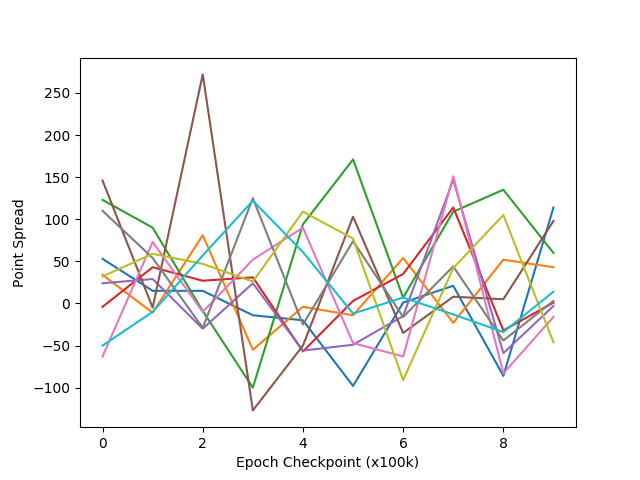
\includegraphics[width=\textwidth]{images/discussion/usefulness/r2-time-series-9.png}
	\caption{Point spreads for 9-game matches} %, like in human play.}
	\label{fig:r2-time-series-9}
\end{subfigure}
~
\begin{subfigure}[b]{0.45\textwidth}
	\center
	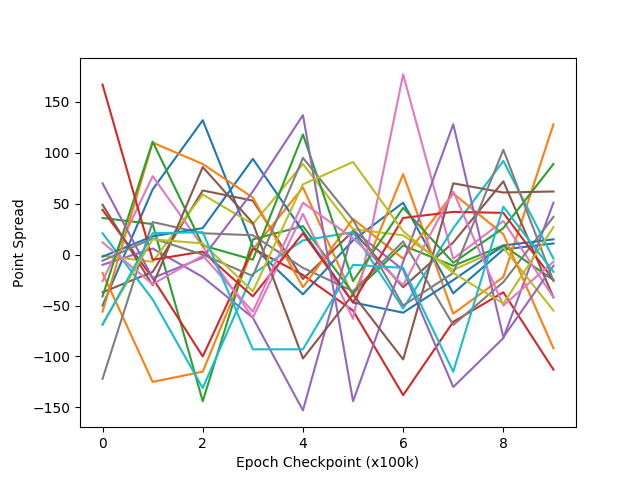
\includegraphics[width=\textwidth]{images/discussion/usefulness/r2-time-series-100.png}
	\caption{Point spreads for 100-game matches.}
	\label{fig:r2-time-series-100}
	% TODO: ^^^ make sure we have an accurate graph,
	%		scale leads me to believe we have the wrong graph
\end{subfigure}

\begin{subfigure}[b]{0.66\textwidth}
	\center
	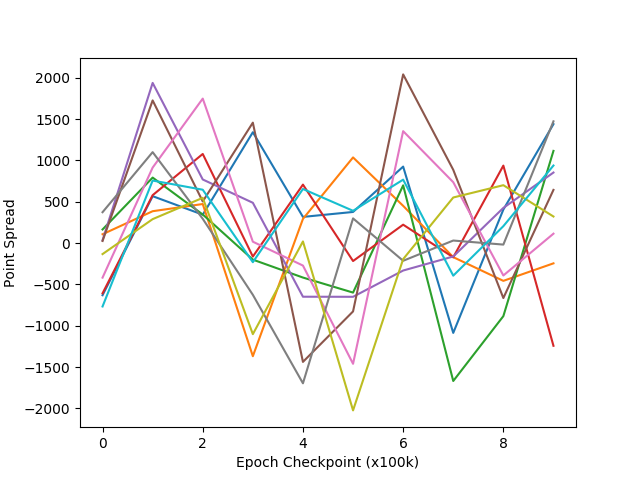
\includegraphics[width=\textwidth]{images/discussion/usefulness/r2-time-series-1000.png}
	\caption{Point spreads for 1,000-game matches.}
	\label{fig:r2-time-series-1000}
\end{subfigure}

\begin{subfigure}[b]{0.66\textwidth}
	\center
	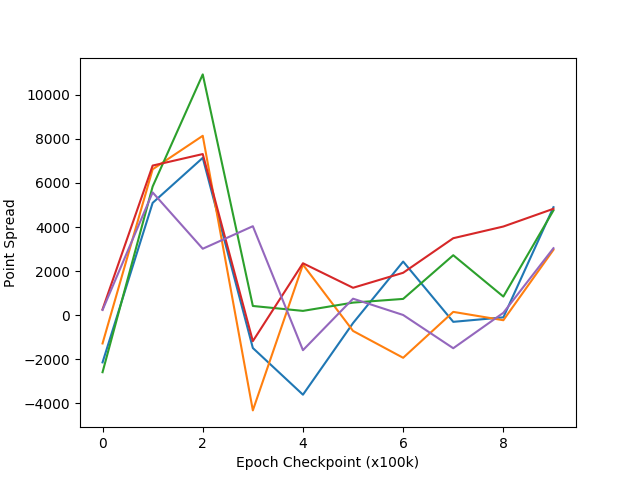
\includegraphics[width=\textwidth]{images/discussion/usefulness/r2-time-series-10000.png}
	\caption{Point spreads for 10,000-game matches.}
	\label{fig:r2-time-series-10000}
\end{subfigure}

\caption{
	Point spreads across matches of varying lengths.
	In each graph,
	the final \learned\ agent is played against its previous checkpoint
	iterations.
}
\label{fig:r2-time-series}
\end{figure}
